%TODO Can you make this a separate document with title and authors, and explain at the start what this document contains. Two figures could fit on one page so this looks a bit more organised and optimised. Captions I think also go at the end of the main text for some reason. Please have a look at the author guidelines. Once I have summary, can draft coverletter. Will then also read one more time.


\documentclass[10pt,letterpaper]{article}
%\documentclass[10pt]{article}
%\usepackage[top=0.85in,left=2.75in,footskip=0.75in]{geometry}

\usepackage[paper=a4paper,
  inner=2.5cm,
  outer=3.8cm,
  bindingoffset=.5cm,
  top=1.5cm,
  bottom=1.5cm]{geometry}


% amsmath and amssymb packages, useful for mathematical formulas and symbols
\usepackage{amsmath,amssymb}
\usepackage{physics}
\newcommand{\pdvn}[3]{\frac{\partial^{#1} {#2}}{\partial {#3}^{#1}}}
\newcommand{\Underbrace}[2]{{\underbrace{#2}_{#1}}}

% Use adjustwidth environment to exceed column width (see example table in text)
\usepackage{changepage}

% Adjusts space between float and caption
\usepackage{caption}
\captionsetup{skip=10pt}  

% textcomp package and marvosym package for additional characters
\usepackage{textcomp,marvosym}

% cite package, to clean up citations in the main text. Do not remove.
% \usepackage{cite}

% Use nameref to cite supporting information files (see Supporting Information section for more info)
\usepackage{nameref,hyperref}

% line numbers
\usepackage[right]{lineno}

% ligatures disabled
\usepackage[nopatch=eqnum]{microtype}
\DisableLigatures[f]{encoding = *, family = * }

% color can be used to apply background shading to table cells only
\usepackage[table]{xcolor}

% array package and thick rules for tables
\usepackage{array}

% create "+" rule type for thick vertical lines
\newcolumntype{+}{!{\vrule width 2pt}}

% create \thickcline for thick horizontal lines of variable length
\newlength\savedwidth
\newcommand\thickcline[1]{%
  \noalign{\global\savedwidth\arrayrulewidth\global\arrayrulewidth 2pt}%
  \cline{#1}%
  \noalign{\vskip\arrayrulewidth}%
  \noalign{\global\arrayrulewidth\savedwidth}%
}


% \thickhline command for thick horizontal lines that span the table
\newcommand\thickhline{\noalign{\global\savedwidth\arrayrulewidth\global\arrayrulewidth 2pt}%
\hline
\noalign{\global\arrayrulewidth\savedwidth}}


% Remove comment for double spacing
\usepackage{setspace} 
\doublespacing

% Text layout
\raggedright
\setlength{\parindent}{0.5cm}
\textwidth 5.25in
\textheight 8.75in

% Bold the 'Figure #' in the caption and separate it from the title/caption with a period
% Captions will be left justified
\usepackage[aboveskip=1pt,labelfont=bf,labelsep=period,justification=raggedright,singlelinecheck=off]{caption}
\renewcommand{\figurename}{Fig}
  
% Use the PLoS provided BiBTeX style
% \bibliographystyle{plos2015}
% Remove brackets from numbering in List of References

\makeatletter
\renewcommand{\@biblabel}[1]{\quad#1.}
\makeatother




% Header and Footer with logo

\usepackage{lastpage,fancyhdr,graphicx}
\usepackage{epstopdf}
\usepackage[bibstyle=numeric,style=authoryear-icomp,maxbibnames=10,maxcitenames=2,uniquelist=false, backend=bibtex,url=false, sorting=none]{biblatex}
\usepackage{float}



\addbibresource{manual.bib}
\AtEveryBibitem{\clearfield{note}}



\pagestyle{fancy}
\fancyhf{}

\rfoot{\thepage/\pageref{LastPage}}
\renewcommand{\headrulewidth}{0pt}
\renewcommand{\footrule}{\hrule height 2pt \vspace{2mm}}
\fancyheadoffset[L]{2.25in}
\fancyfootoffset[L]{2.25in}
\lfoot{\today}

%% Include all macros below

\newcommand{\lorem}{{\bf LOREM}}
\newcommand{\ipsum}{{\bf IPSUM}}

%% END MACROS SECTION

\setlength{\parskip}{\baselineskip}%
\setlength{\parindent}{0pt}%
\begin{document}
\vspace*{0.2in}

% Title must be 250 characters or less.
\begin{flushleft}
{\Large
\textbf\newline{Effects of multistability, absorbing boundaries and growth on Turing pattern formation} % Please use "sentence case" for title and headings (capitalize only the first word in a title (or heading), the first word in a subtitle (or subheading), and any proper nouns).
}
\newline
% Insert author names, affiliations and corresponding author email (do not include titles, positions, or degrees).
\\
Martina Oliver Huidobro \textsuperscript{1},
Robert G. Endres \textsuperscript{1}


\bigskip
\textbf{1} Department of Life Sciences and Centre for Integrative Systems Biology and Bioinformatics, Imperial College, London, United Kingdom
\\
\bigskip

* r.endres@imperial.ac.uk

\end{flushleft}

% \printbibliography[heading=bibintoc]


\section*{Supplementary Material}

This supplementary material contains figures and tables with parameters which are referenced throughout the main text and supports the research findings.

\newcommand{\beginsupplement}{%
    \setcounter{table}{0}
    \renewcommand{\thetable}{S\arabic{table}}%
    \setcounter{figure}{0}
    \renewcommand{\thefigure}{S\arabic{figure}}%
}
\beginsupplement

\begin{figure}[!ht]
    \center
    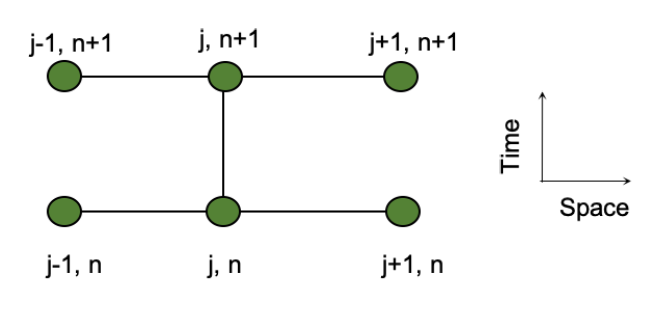
\includegraphics[width=0.6\textwidth]{figures/stencils}

    \caption{{\bf Crank–Nicolson (CN) algorithm for numerical solution.}  Geometric representation (stencil) with nodes and edges that represent the points of interest for the numerical approximation. The points of interest, which are the ones present in the equations, are shown in green. Labels $j$ and $n$ are the current space and time points. The CN stencil has one spatial dimension and one temporal dimension, with axes labels time ($t$) and space ($x$). }   \label{sup_fig1}
\end{figure}


\begin{figure}[H]
    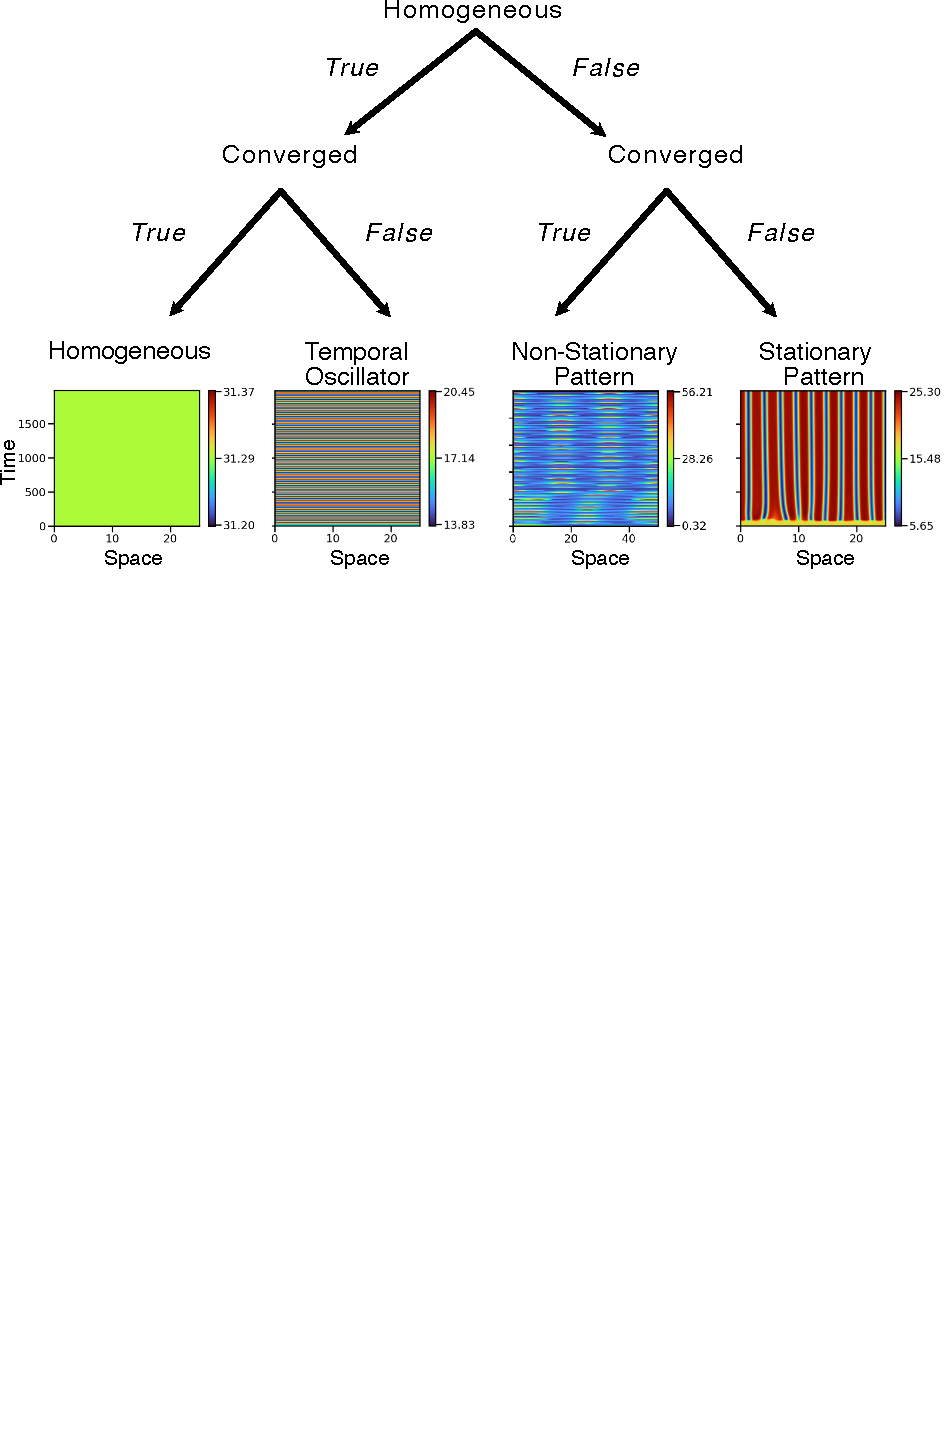
\includegraphics[width=1\textwidth]{figures/no_growth_classification}
    \vspace{5pt}
    \caption{{\bf Decision tree for pattern classification in non-growing domains with reflective boundaries}. The decision tree is based on two layers: spatial homogeneity and convergence. The numerical solutions for the four different pattern outcomes include homogeneous, temporal oscillator, non-stationary, and stationary patterns as in the bottom. In the four numerical solutions, time is in the $y$ axis, space in the $x$ axis, and concentration in the colorbar.}
    \label{sup_fig2}
\end{figure}


\begin{figure}[H]
    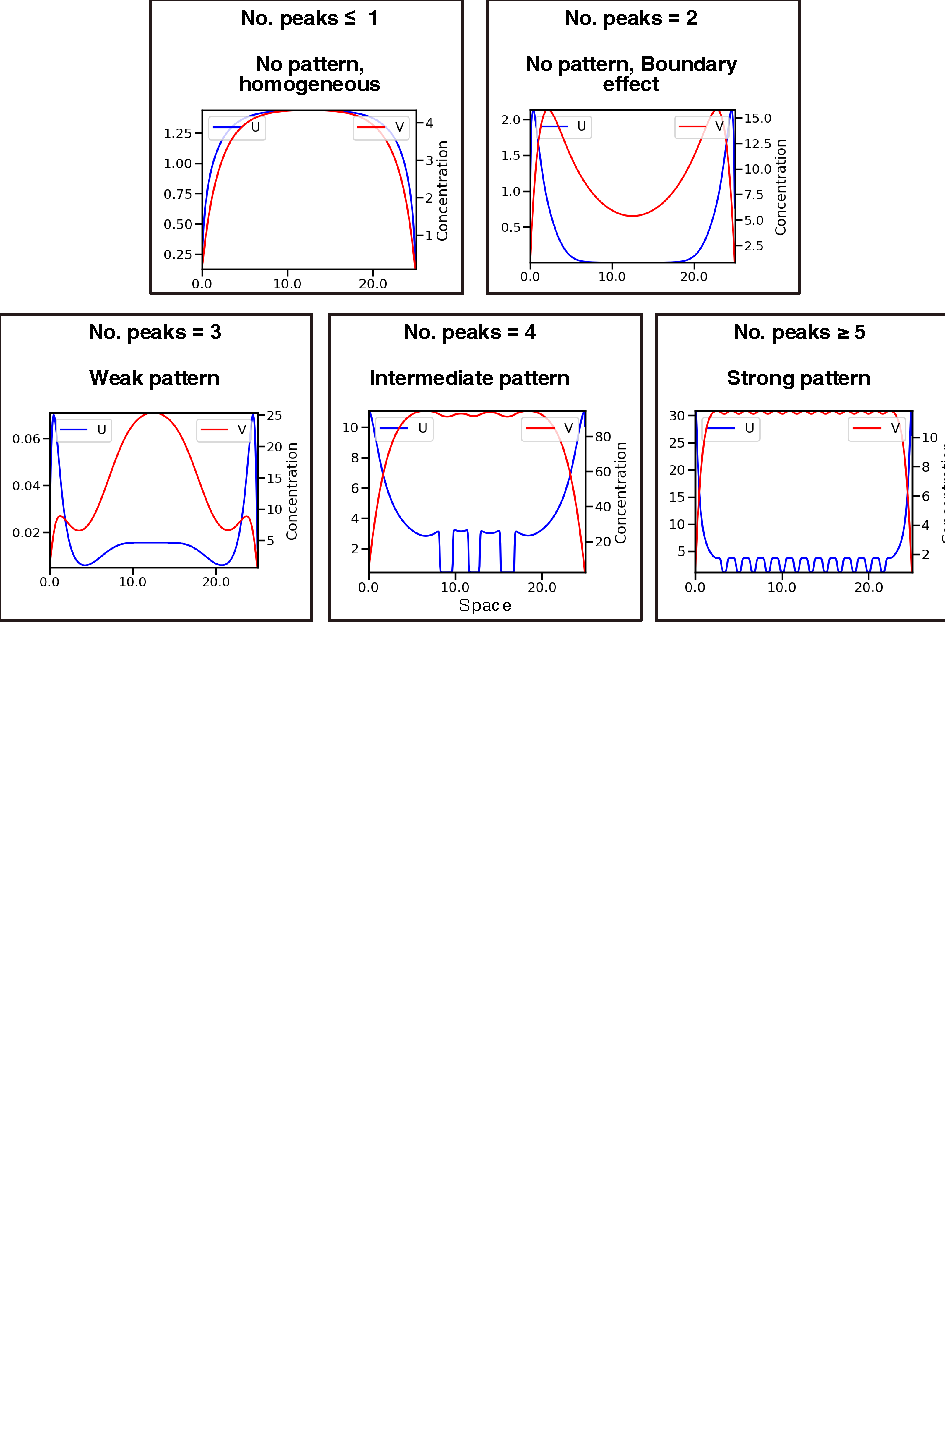
\includegraphics[width=1\textwidth]{figures/growth_classification}
    \vspace{5pt}

    \caption{{\bf Pattern classification with absorbing boundaries.} Patterns are classified according to the number of peaks as shown in the 5 cases of this figure.}
    \label{sup_fig3}
\end{figure}


\begin{figure}[H]
    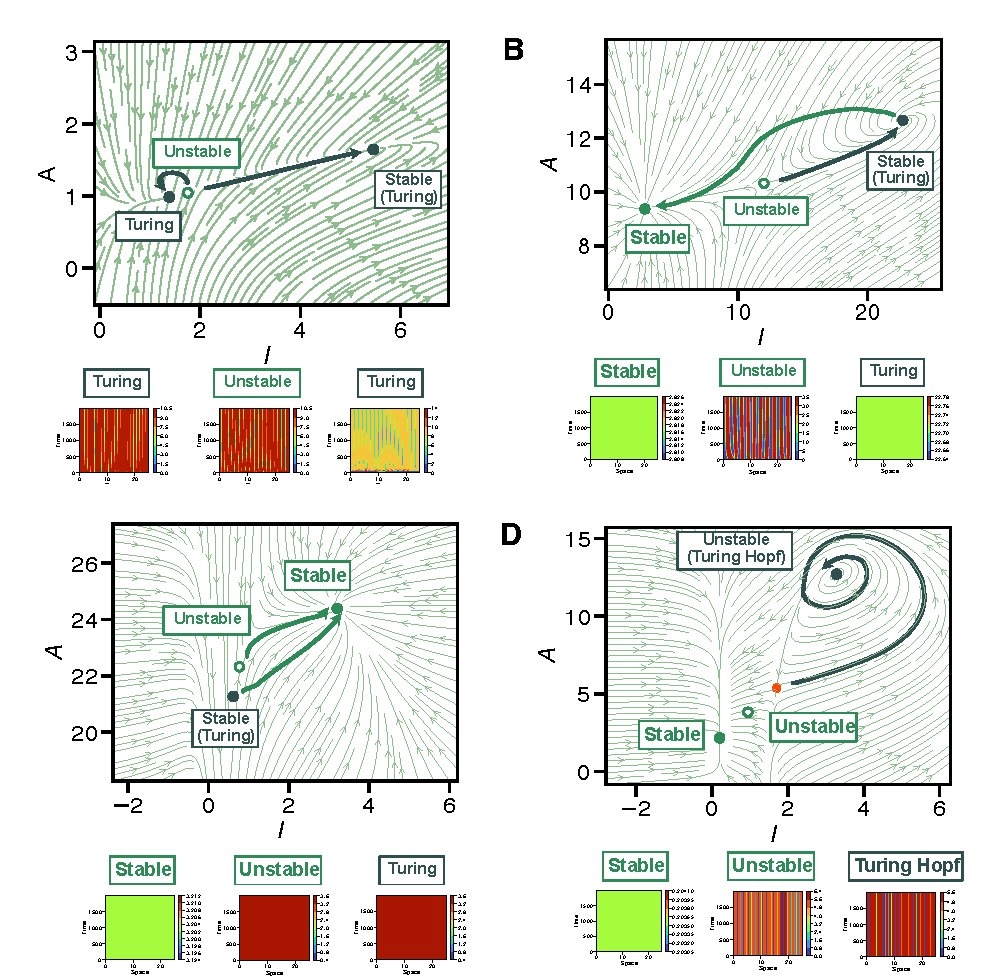
\includegraphics[width=1\textwidth]{figures/multistability_leftovers}
    \vspace{5pt}

    \caption{{\bf Other types of multistability dynamics.} \textbf{(A)} Unstable state converges into Turing. \textbf{(B)} Unstable state produces pattern, while Turing state loses pattern. \textbf{(C)} Multistability disrupts all patterns. \textbf{(D)} Turing I Hopf state attracts the unstable state and generates a pattern.}

    \label{sup_fig4}
\end{figure}




\begin{figure}[H]
    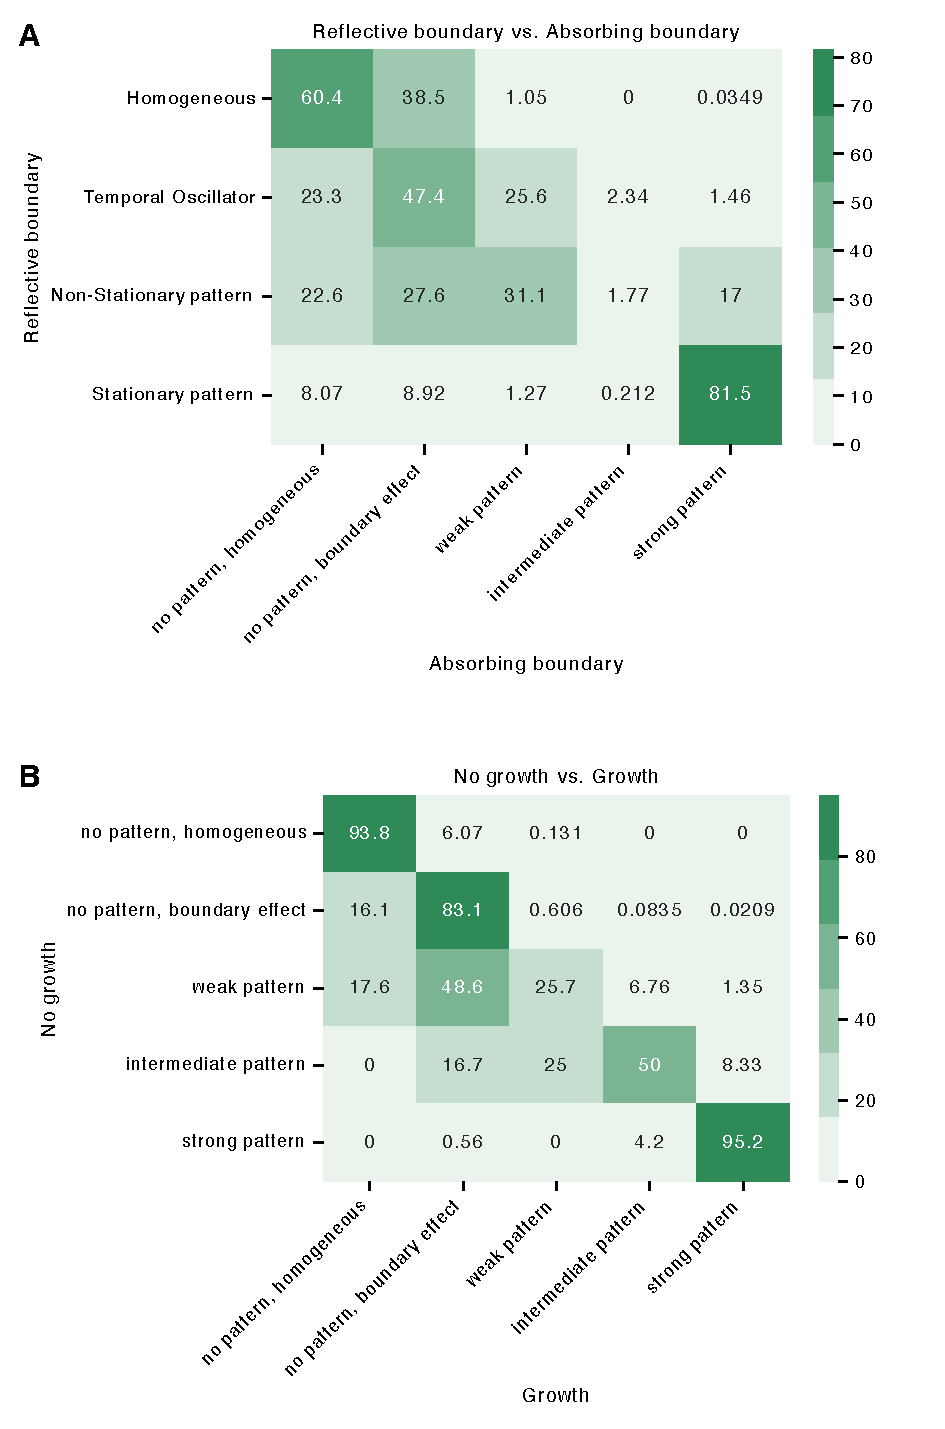
\includegraphics[width=1\textwidth]{figures/sup_confusion_matrix}

    \caption{{\bf Confusion matrix for pattern transitions.} \textbf{(A)} Numerical outcome of reflective boundaries ($y$ axis) versus absorbing boundaries ($x$ axis).\textbf{(B)} Numerical outcome of non-growing domains ($y$ axis) versus growing-domains ($x$ axis). Numbers show the percentage of solutions across the row.}

    \label{sup_fig5}
\end{figure}



\begin{table}[H]
    \centering
    \renewcommand{\arraystretch}{1.3} % Adjust vertical padding
    \begin{tabular}{|c|c|c|c|c|}
        \hline
        \textbf{Parameter} & \textbf{Distribution} & \textbf{Value 1} & \textbf{Value 2} & \textbf{Value 3} \\
        \hline
        $V_{m}$ & Loguniform & (10, 1000) & (10, 10000) & (10, 10000) \\
        \hline
        $K_{m}$ & Loguniform & (0.1, 250) & (0.1, 100) & (0.1, 100) \\
        \hline
        $\mu_{m}$ & Loguniform & (0.001, 50) & (1, 100)& (1, 100) \\
        \hline
        $D_{B}$ & Loguniform / Fixed & (0.001, 10) & 0.01 & 10 \\
        \hline
        $D_{A}$ & Fixed & 1 & 10 & 0.01 \\
        \hline
        $b$ & Fixed / Loguniform & 0.01 & (10, 10000) &  (10, 10000) \\
        \hline
        $n$ & Fixed / Loguniform & 2 & (2, 4) & (2, 4) \\
        \hline
    \end{tabular}
        \vspace{10pt}

    \caption{\textbf{Kinetic parameters for PDE system.} A combination of the three values is used throughout this study to obtain a wide range of dynamical behaviors.}
    \label{tab:sup_table1}
\end{table}




\begin{table}[H]
    \centering
    \renewcommand{\arraystretch}{1.3} % Adjust vertical padding
    \begin{tabular}{|c|c|c|c|c|}
        \hline
        \textbf{Parameter} & $L$ & $\Delta x$ & $T$ & $\Delta t$ \\
        \hline
        \textbf{Value 1} & 25 & 0.05 & 2000 & 0.005 \\
        \hline
        \textbf{Value 2} & 100 & 0.2 & 18000 & 0.05 \\
        
        \hline
    \end{tabular}
    \vspace{10pt}
    \caption{\textbf{System parameters for numerical simulation}.Value 1 parameters are used for Figs 1,2,3,4 as well as Fig S2,Fig S3,Fig S4. Value 2 parameters are used for Fig 5 and Fig S5.}
    \label{tab:sup_table2}
\end{table}



\end{document}

